\documentclass{article}
\usepackage{graphicx}
\usepackage{hyperref}
\usepackage{float}
\usepackage{multicol}

\title{Practica 1: Entorno y Lenguaje de Programacion}

\author{Adolfo Roman Jimenez}

\begin{document}
	
	\maketitle
	
	\section{Objetivo}
	
	Identificar y probar el entorno de ejecución y el lenguaje de programación orientado a	objetos a utilizar durante el curso.
	
	\section{Actividades}
	
	\begin{itemize}
		\item Probar los conceptos basicos del entorno y lenguaje
		\item Revisar la instalacion y configuracion del entorno de ejecucion
		\item Realizar un programa en el lenguaje de programación usando el entorno de ejecución, utilizando la sintaxis básica (notación, palabras reservadas, comentarios, etc.) 
	\end{itemize}
	\newpage
	
	\section{Manual de Practicas - Desarrollo}
	
	\subsection{Instalacion}
	
		\subsubsection{Java Virtual Machine (JVM) y Programas en Java}
		
		La Maquina Virtal de Java, compila y ejecuta el programa que a diferencia de otros lenguajes de programacion, no se ejecuta directamente en el sistema, sino dentro de la propia maquina virtual.\\
		
		Por ejemplo, en el lenguaje de programacion C, se pueden crear funciones en bibliotecas distintas que se compilan creando archivos \verb*|.obj| y que despues el mismo compilador combina en un unico archivo \verb*|.out| o \verb*|.exe| que es el programa que contiene el lenguaje de maquina que ejecutara el sistema operativo.
		
		\begin{figure}[H]
			\centering
			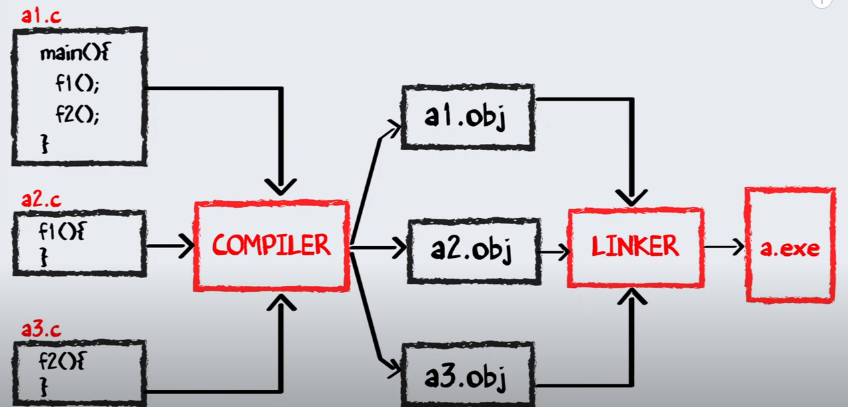
\includegraphics[scale = 0.3]{images/comp}
			\caption{Proceso de compilacion en C}
		\end{figure}
		
		En el caso de Java, el proceso de compilacion y ejecucion primeramente se lleva a cabo cuando guardamos algun archivo con la extension \verb*|archivo.java|. Despues, al momento de compilar, se genera el \verb*|archivo.class| que es lo que Java usa para ejecutar dentro del JVM. 
		
		\begin{figure}[H]
			\centering
			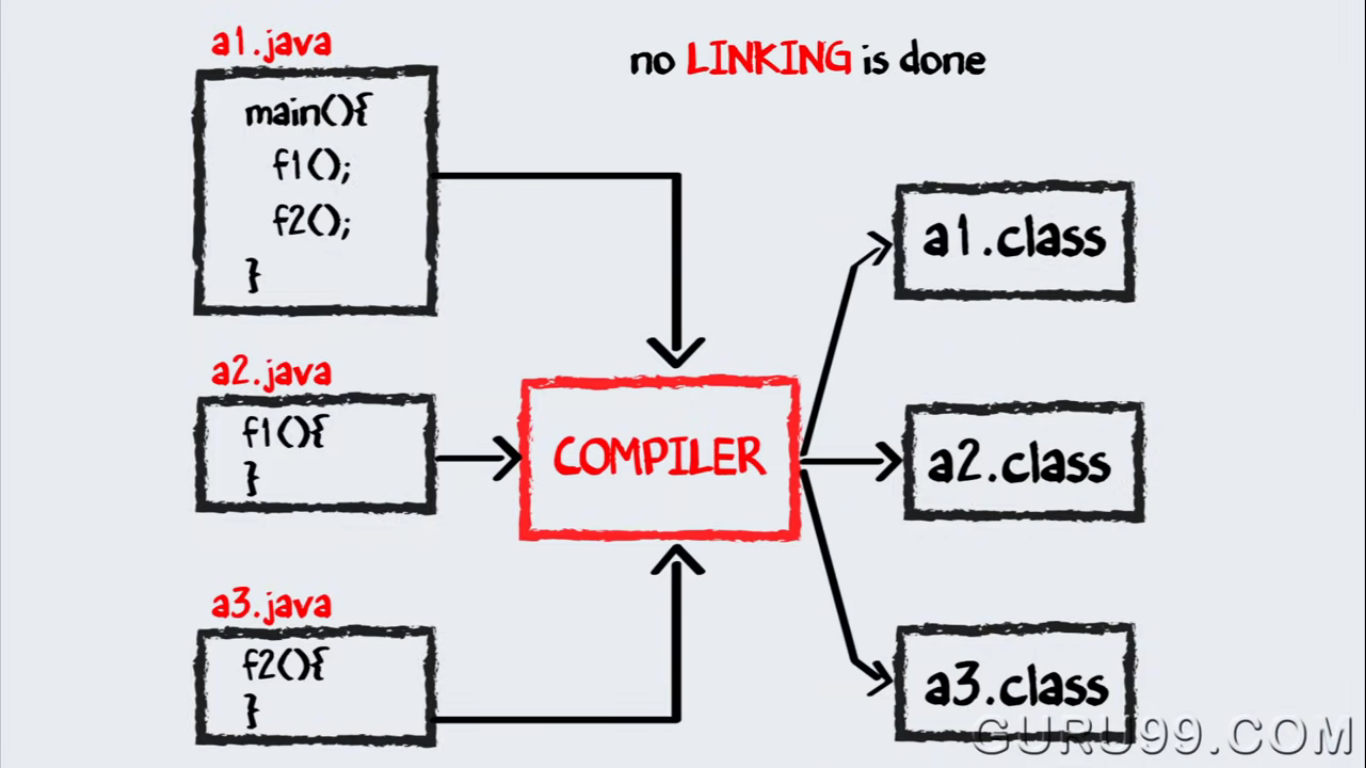
\includegraphics[scale = 0.18]{images/javacomp1}
			\caption{Proceso de compilacion en Java}
		\end{figure}
	
		Despues de esto, los archivos \verb*|.class| no se mezclan para formar un ultimo archivo ejecutable, sino que se transmiten a la \emph{Java Virtual Machine} que dentro de su propio entorno, carga primero los archivos \verb*|.class| para posicionarlos en el \emph{heap} de la memoria, mientras sus instancias las deposita en el \emph{stack}. Este programa se va convirtiendo en \emph{bytecode} que despues el \emph{JIT} dentro la maquina virtual convertira en lenguaje de maquina ejecutable.
		
		\begin{figure}[H]
			\centering
			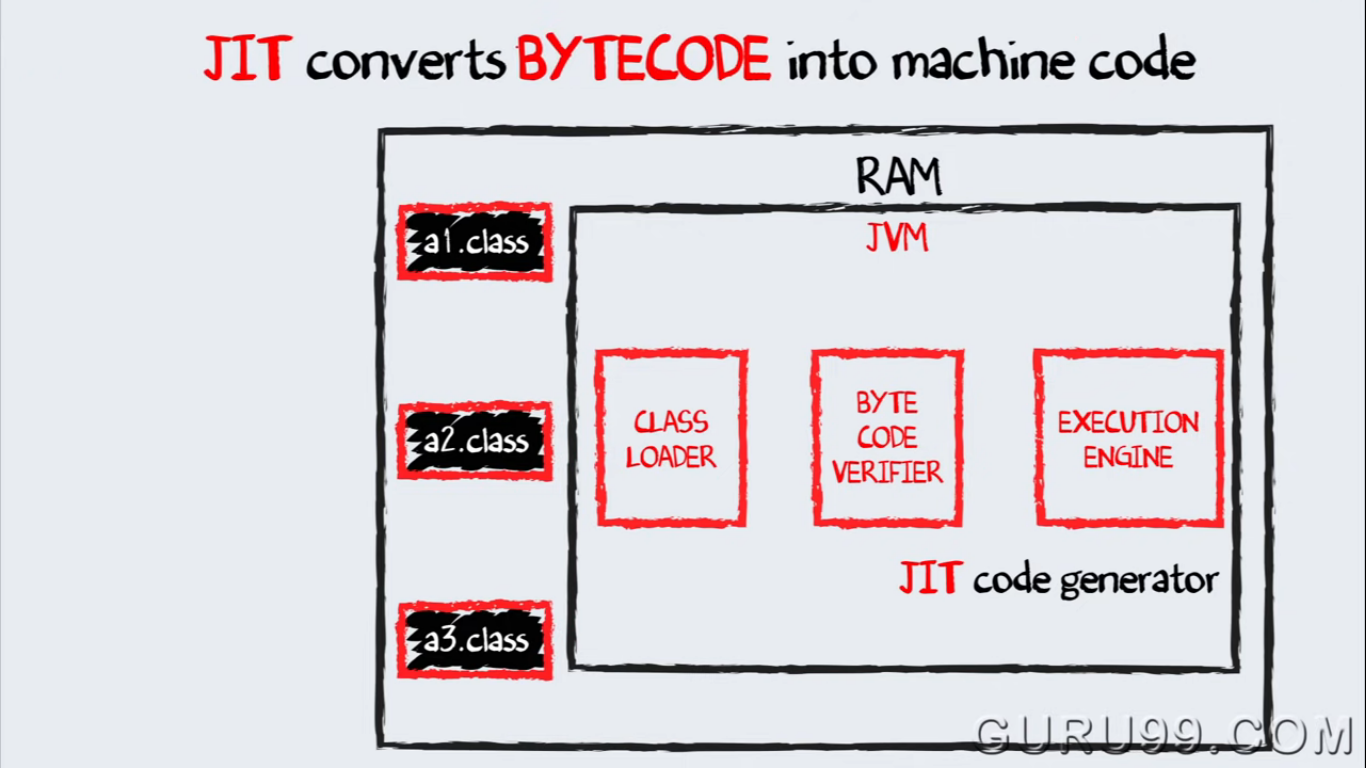
\includegraphics[scale = 0.2]{images/javacomp2}
			\caption{Proceso de compilacion en Java}
		\end{figure}
		\newpage
	
		\subsubsection{Herramientas de Desarrollo (JDK)}
		
		Las herramientas de desarrollo en Java \emph{(Java Development Kit)} proporcionan el entorno de desarrollo que usaremos para poder programar en Java. En mi caso usaremos el kit de desarrollo \emph{Amazon Coretto 11} que es bastante usado debido a la popularidad de \emph{Amazon Web Services}. 
		
		\begin{figure}[H]
			\centering
			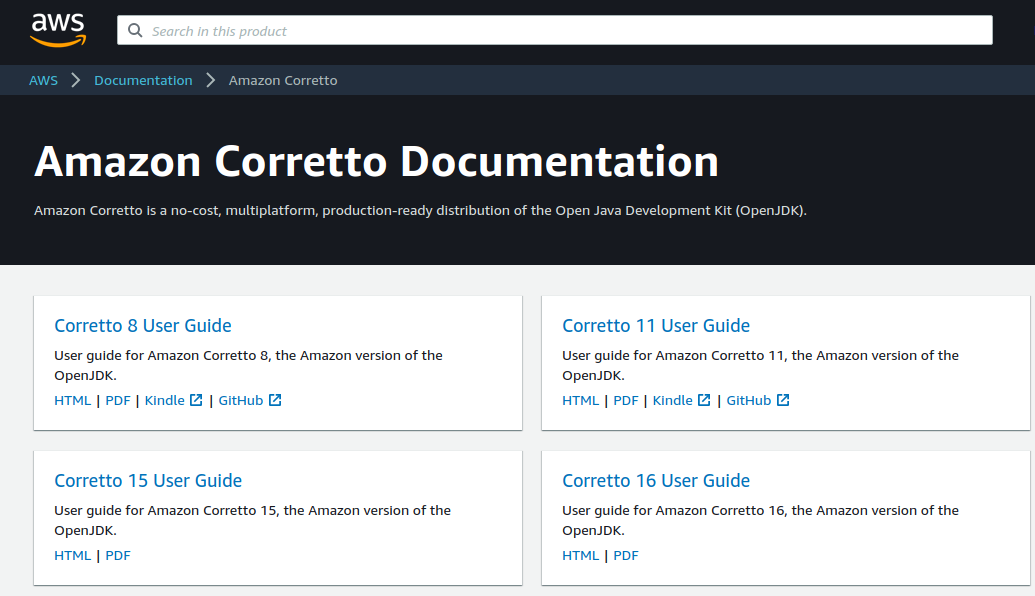
\includegraphics[scale = 0.35]{images/corettodoc}
			\caption{Pagina web de Amazon Coretto}
		\end{figure}
	
		Despues de instalar \emph{Amazon Coretto 11} en la computadora, verificamos que la instalacion.
		
		\begin{figure}[H]
			\centering
			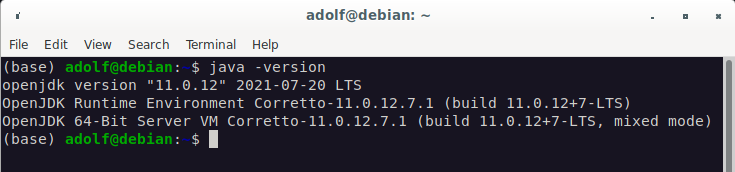
\includegraphics[scale = 0.55]{images/terminaljdk}
			\caption{Amazon Coretto 11 instalado en Debian 11}
		\end{figure}

	\subsection{Programando en Java}
	
		\subsubsection{Codificacion}
		
			Usando el editor \emph{Atom} creamos nuestro primer programa \verb*|HolaMundo.java|.
			
			Es importante que el nombre del archivo sea exactamente el mismo que el de la clase con la que se trabaja, pues de lo contrario el compilador nos mostrara un error al momento de ejecutarlo.
			
			\begin{figure}[H]
				\centering
				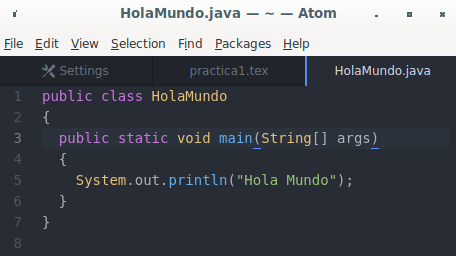
\includegraphics[scale = 0.8]{images/holamundo}
				\caption{Primer programa en Java con el editor Atom}
			\end{figure}
		
		\subsubsection{Compilacion y Programacion}
		
			Despues de escribir el programa, procedemos a compilarlo con el \emph{JDK} que acabamos de instalar.\\
			
			El comando para compilar es \verb*|javac| seguido del nombre del archivo con la extension \verb*|.java|.\\
			
			Si la compilacion fue exitosa, el programa no nos mostrara ningun tipo de error y acto seguido podremos apreciar que se crea un archivo del mismo nombre que nuestro archivo original pero ahora con una extension \verb*|.class| que para ejecutarla, lo unico que debemos de hacer es ingresar el comando \verb*|java| y despues de este el nombre del archivo \verb*|.class| pero sin la extension como se muestra en la siguiente imagen.
			
			\begin{figure}[H]
				\centering
				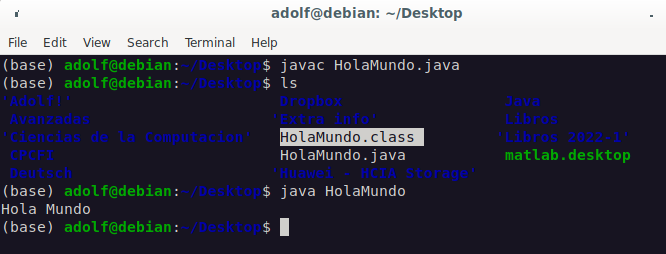
\includegraphics[scale = 0.5]{images/holamundocomp}
				\caption{Compilacion y Ejecucion de HolaMundo en Java}
			\end{figure}
		
		\subsubsection{Entorno de Desarrollo Integrado (IDE)}
		
		El entorno de desarrollo integrado \emph{(Integrated Development Environment)} es un programa que amplia las herramientas para desarrolladores del lenguaje bajo el que se trabaje y que tambien provee de entornos de ejecucion y correcion de software integrados dentro del mismo programa, lo cual hace de un IDE una herramienta que simplemente facilita el trabajo del desarrollador al tener la mayoria o todas las opciones necesarias a la mano dentro un mismo entorno.\\
		
		En mi caso preferi utilizar el entorno \emph{IntelliJIDE} debido a que me parecio el mas adecuado para mi sistema operativo.
		
		\begin{figure}[H]
			\centering
			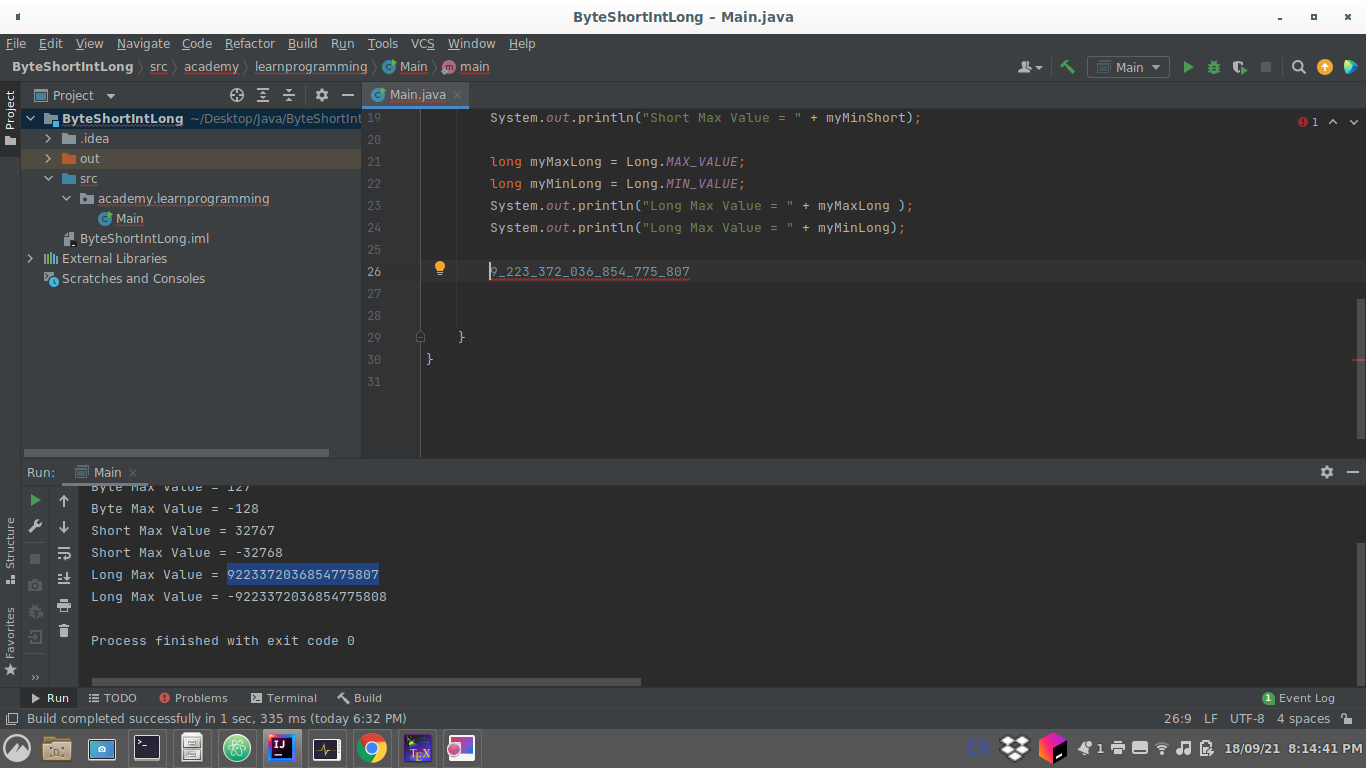
\includegraphics[scale = 0.25]{images/ide}
			\caption{IntelliJIDE para Debian 11}
		\end{figure}
	
	\subsection{Estructura de un Programa en Java}
	
		\subsubsection{Estructura de Clase}
		
		Como ya se habia mencionado, un programa en Java para que pueda compilar correctamente, inicialmente debe de tener una clase que se llame de la misma forma que el archivo.\\
		
		La clase principal debe ser publica y debe de contener un metodo \emph{main} junto con el identificador \emph{class}.
		
		\begin{figure}[H]
			\centering
			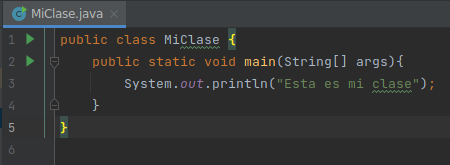
\includegraphics[scale = 0.8]{images/miclase}
			\caption{Programa con clase de nombre "MiClase" en IntelliJIDEA}
		\end{figure} 
		
		Al compilar el programa podemos ver que el programa se ejecuta de forma correcta en el IDE.
		
		\begin{figure}[H]
			\centering
			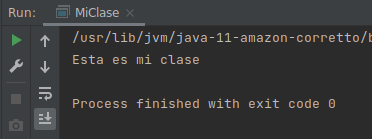
\includegraphics[scale = 1]{images/miclase2}
			\caption{Ejecucion de "MiClase" en IntelliJIDEA}
		\end{figure} 
		
		\begin{figure}[H]
			\centering
			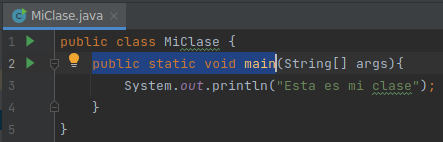
\includegraphics[scale = 0.8]{images/miclasemain}
			\caption{Contenido de "main" en la clase principal}
		\end{figure} 
	
		\subsubsection{Comentarios}
		
		Existen diversas formas de insertar comentarios en un programa de Java para indicar sobre diversos temas, ya sea como instrucciones e indicaciones para los programadores que no conozcan el programa o como informacion sobre la autoria de este, credenciales, permisos, etc.
		
		\begin{figure}[H]
			\centering
			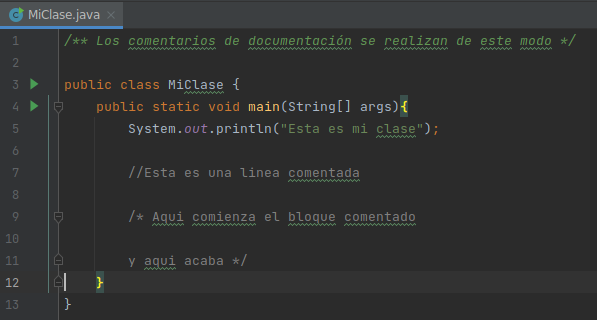
\includegraphics[scale = 0.6]{images/miclasecoments}
			\caption{Comentarios dentro de clase "MiClase"}
		\end{figure} 
		\newpage
	
		\subsubsection{Palabras Reservadas}
		
	 	Similar a los lenguajes que ya se han usado en el pasado, el lenguaje de Java, tambien tiene una serie de palabras que estan reservadas y no se pueden usar, pues corresponden a la sintaxis del lenguaje como tal.
	 	
	 	Estas palabras incluyen fundamentalmente metodos y tipos de datos que el lenguaje usa para su correcto funcionamiento.
	 	
	 	\begin{figure}[H]
	 		\centering
	 		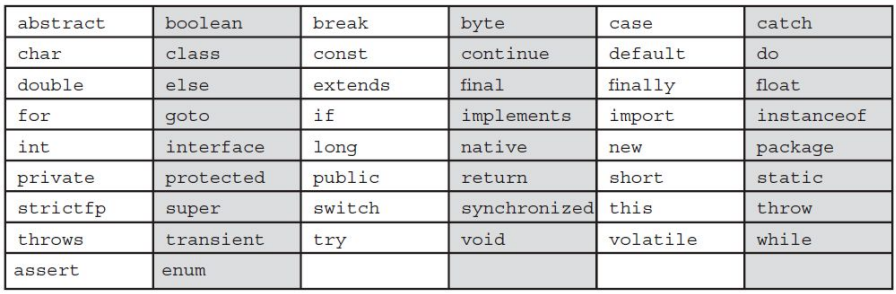
\includegraphics[scale = 0.4]{images/words}
	 		\caption{Set de Palabras Reservadas en Java}
	 	\end{figure} 
 		\newpage
 	
 	\section{Practica Sugerida - Desarrollo}
 	
 		\subsection{Ejercicio 1}
 		
 		Para este ejercicio se nos pide instalar el \emph{JDK} de \emph{Oracle} recomendado en la practica. Sin embargo, yo decidi instalar \emph{Amazon Coretto 11} ya que me se adecua mejor al sistema operativo que tengo.
 		
 		\begin{figure}[H]
 			\centering
 			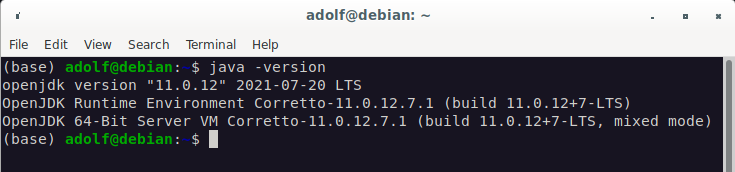
\includegraphics[scale = 0.6]{images/terminaljdk}
 			\caption{JDK, Amazon Coretto 11}
 		\end{figure} 
 	
 		\subsection{Ejercicio 2}
 		
 		En este ejercicio debemos de escribir un programa que pida al usuario 2 numeros y que de estos numeros imprima la suma, el producto, la diferencia y el cociente de estos.\\
 		
 		Para lograrlo, importe la biblioteca \emph{Scanner} que me permitio al momento de declararla, crear una instancia llamada simplemente \emph{scan} con la cual utilice el metodo \emph{nextInt()} para obtener los inputs del usuario.\\
 		
 		Antes de cada solicitud de \emph{input} imprimi una leyenda con \verb*|System.out.println| solicitando al usuario ingresar un numero en cada de los requerimientos y el resultado lo deposite en dos variable de tipo int \textbf{a} y \textbf{b} respectivamente.\\
 		
 		Despues con la ayuda de nuevo de \verb*|System.out.println| simplemente indique que era el tipo de resultado que se estaba imprimiendo y realice la operacion dentro de la misma linea a imprimir como argumento. En el caso del promedio entre dos enteros, tuve que hacer un \emph{cast} de ambos tipos de dato entero para que el resultado pudiera presentarse como un numero no entero.
 		
 		\begin{figure}[H]
 			\centering
 			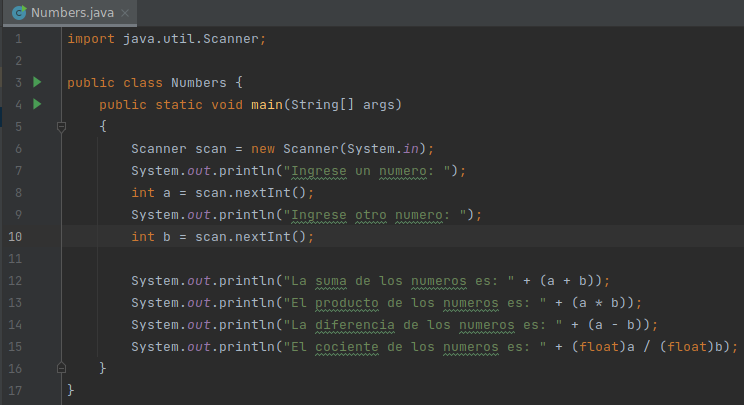
\includegraphics[scale = 0.5]{images/numbers}
 			\caption{Codigo en IntelliJIDE del Ejercicio 1}
 		\end{figure}
 	
 		\begin{figure}[H]
 			\centering
 			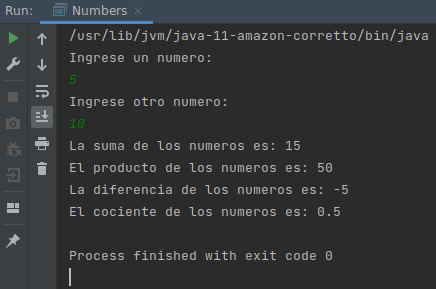
\includegraphics[scale = 0.75]{images/numbersout}
 			\caption{Ejecucion del ejercicio dentro del IDE}
 		\end{figure}  
 		
 		\subsection{Ejercicio 3}
 		
 		Para este ejercicio que nos pedia imprimir una serie de asteriscos en forma de cuadrado, ovalo, flecha y diamante, simplemente utilize distintos comandos \verb*|System.out.println| para linea por linea, imprimir la forma solicitada y que el resultado fuera similar al requerido por la practica.
 		
 		\begin{figure}[H]
 			\centering
 			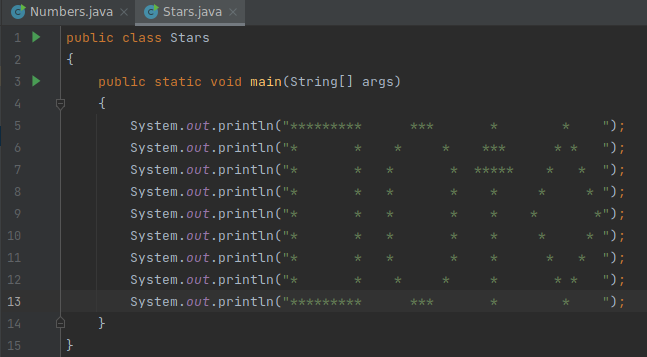
\includegraphics[scale = 0.5]{images/stars}
 			\caption{Hard-coding de las figuras solicitadas}
 		\end{figure}
 	
 		\begin{figure}[H]
 			\centering
 			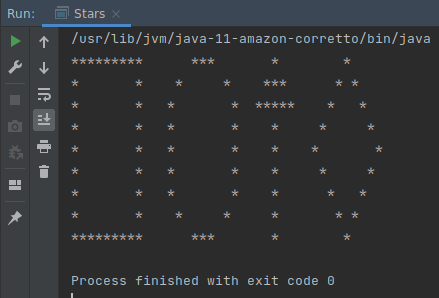
\includegraphics[scale = 0.6]{images/starsout}
 			\caption{Output del ejercicio 3}
 		\end{figure}
 		
 		\subsection{Ejercicio 4}
 		
 		En este ejercicio que fue similar al ejercicio 2, tuve que importar un par de clases adicionales para poder escoger el numero minimo y numero maximo que el ejercicio solicita que fueron las librerias \emph{Arrays} y \emph{Collections}.\\
 		
 		La clase \emph{Arrays} contiene diversos metodos para manipular arreglos, como de ordenamiento o de busqueda y la clase \emph{Collections} contiene metodos estaticos que operan y regresan colleciones de elementos.\\
 		
 		Declare la clase \emph{Scanner} al principio del programa tambien y despues utilice la instancia \emph{scan} para solicitar a usuario las 3 variables enteras requeridas.\\
 		
 		Despues de que el usuario ingresa las variables y las deposito dentro de las variables enteras \textbf{a},\textbf{b} y \textbf{c}, creo un arreglo de enteros con la clase \emph{Integer} y deposito ahi el valor de las variables obtenidas como elementos del arreglo.\\
 		
 		Una vez esto, creo dos varibales enteras para obtener el numero minimo y maximo del arreglo \textbf{min} y \textbf{max} y las igualo a los siguiente comandos dependiendo el caso:\\
 		
 		\begin{itemize}
 			\item \verb*|Collections.min(Arrays.asList(arr))|
 			\item \verb*|Collections.max(Arrays.asList(arr))|
 		\end{itemize}
 		
 		Lo que hace cada una de estas directivas, es que la clase \emph{Arrays} genera una lista del arreglo \textbf{arr} y la clase \emph{Collections} aplica el metodo de obtener el valor maximo o valor minimo de esa lista, dependiendo de lo que el programador haya determinado.\\
 		
 		Con respecto al demas funcionamiento del programa, este es similar al del ejercicio 2 como ya lo habiamos mencionado. De igual forma para los distintos \emph{outputs}, declaramos \verb*|System.out.println| y ejecutamos la operacion requerida en alguno de los argumentos de la funcion para que esta imprima el resultado como salida.\\
 		
 		Solo en los casos de valor menor o mayor esto no se da, pues la operacion para determinar que elemento es mayor que el otro, se realiza fuera de las funciones de impresion a pantalla y en estas unicamente se ejecutan los resultados en las variables declaradas.
 		
 		\begin{figure}[H]
 			\centering
 			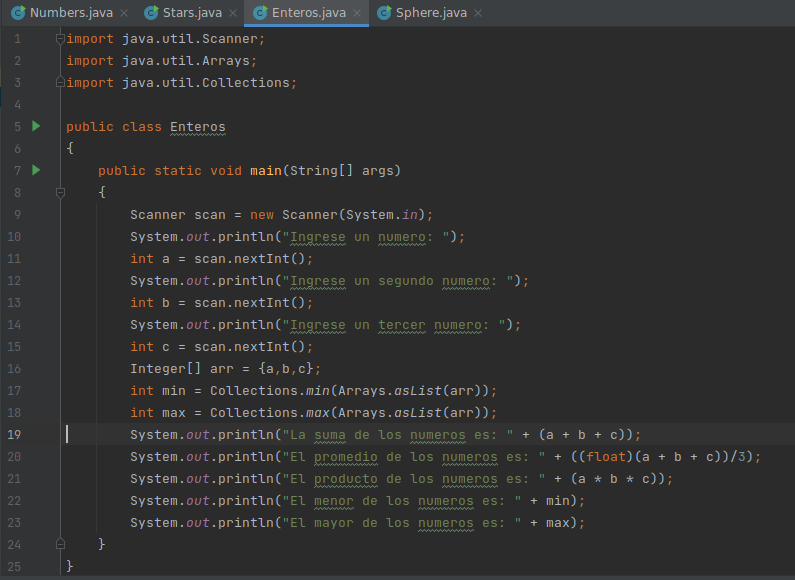
\includegraphics[scale = 0.55]{images/enteros}
 			\caption{Codigo fuente de la clase Enteros para ejercicio 4}
 		\end{figure}
 		
 		\begin{figure}[H]
 			\centering
 			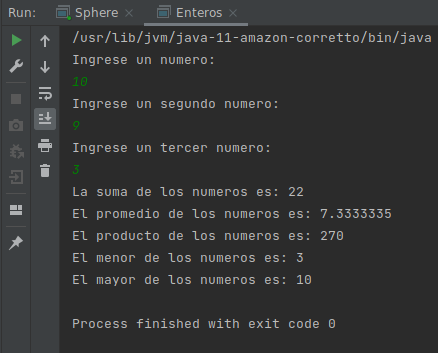
\includegraphics[scale = 0.6]{images/enterosout}
 			\caption{Output de clase Enteros}
 		\end{figure}
 	
 		\subsection{Ejercicio 5}
 		
 		Este ejercicio no fue tan complicado pues es similar a los anteriores en terminos de recopilar datos del usuario y llevar a cabo las operaciones dentro de las funciones de impresion de lineas.\\
 		
 		Algo que lleve a cabo, fue de reducir el numero de decimales a 2 para cualquier tipo de respuesta que involucre numero flotante.\\
 	
 		En cada una de las lineas que imprimen la respuesta, en esta ocasion se usa un metodo diferente que es:\\
 		
 		\verb*|System.out.printf|\\
 		
 		y para el cual, es necesario incluir un salto de linea al final del comando pues esta funcion, no incluye un salto de linea como si lo incluia el metodo \verb*|println|.
 		
 		\begin{figure}[H]
 			\centering
 			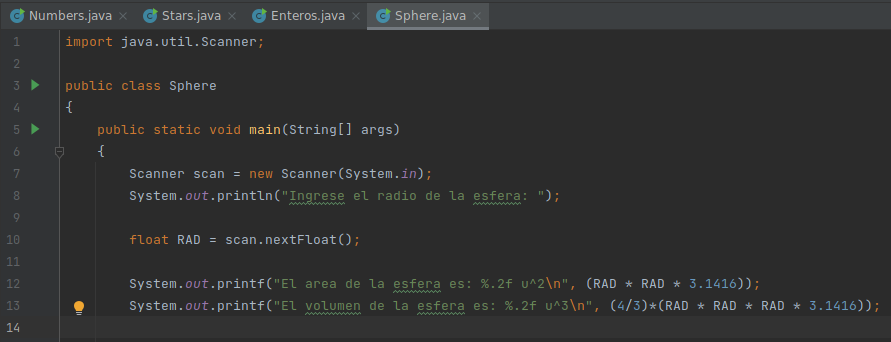
\includegraphics[scale = 0.5]{images/sphere}
 			\caption{Codigo fuente de la clase Sphere}
 		\end{figure}
 		
 		\begin{figure}[H]
 			\centering
 			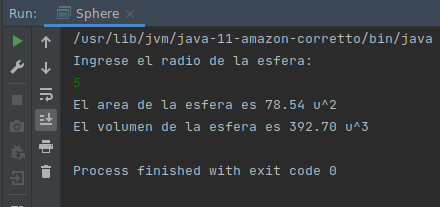
\includegraphics[scale = 0.8]{images/sphereout}
 			\caption{Output de clase Sphere5}
 		\end{figure}
 		\newpage
 	
 	\section{Conclusiones}
 	
 	Me gusto mucho la practica, pues ademas de que es una de las primeros documentos que es escribo en \LaTeX y con el cual me he podido ir acostumbrando a redactar documentos academicos de una mejor manera, tambien aprendi sobre el entorno y el lenguaje de Java.\\
 	
 	Me gusta mucho el \emph{IntelliJ IDEA} pues me parece un entorno bastante amigable y sencillo de usar.\\
 	
 	Por otro lado, en cuanto al lenguaje de Java, me parece que la sintaxis no es tan compleja, pues es muy parecida a la sintaxis de \emph{C} que ya usamos anteriormente, pero creo lo que me emociona en realidad, es la naturaleza del lenguaje que es 100 por ciento orientado a objetos y espero poder aprender mas al respecto durante el semestre.\\
 	
 	Por lo mientras me parece genial que Java contenga diversas clases que podemos importar y funcionan justo como las bibliotecas en \emph{C} o \emph{Python} que por lo regular usamos, pues contienen mucho codigo que podemos utilizar para facilitarnos la vida dentro del lenguaje.\\
 	
 	Me siento emocionado por aprender mas de Java y su funcionalidad como lenguaje Orientado a Objetos. 
 	
 	$\sqrt{2}$ no es un numero racional
 		
 		
 		
 		
 		
		
	
	
	 
			
	
	
	
	
	
	
	
\end{document}